\documentclass{standalone}
\usepackage{tikz}
\usepackage{ctex,siunitx}
\setCJKmainfont{Noto Serif CJK SC}
\usepackage{tkz-euclide}
\usepackage{amsmath}
\usetikzlibrary{patterns, calc,3d}
\usetikzlibrary {decorations.pathmorphing,decorations.pathreplacing,decorations.shapes}
\begin{document}
\small
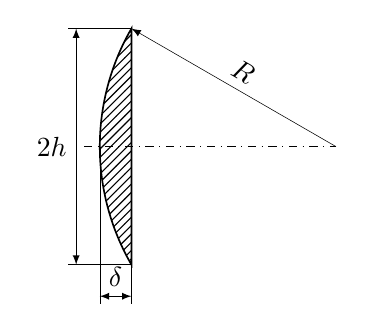
\begin{tikzpicture}[>=latex,scale=1.0]
  \draw[semithick,pattern=north east lines](150:3)arc(150:210:3)--cycle;
  \draw[very thin,->](0,0)--(150:3)node[midway,above,sloped]{$R$};
  \draw[densely dashed,dashdotted](-3.2,0)--(0,0);
  \draw[very thin] (150:3)--++(-0.8,0);
  \draw[very thin] (210:3)--++(-0.8,0);
  \draw[very thin,<->](-3.3,-1.5)--(-3.3,1.5)node[midway,left]{$2h$};
  \draw[very thin](-3,0)--(-3,-2)({-1.5*sqrt(3)},-1.5)--++(0,-0.5);
  \draw[very thin,<->](-3,-1.9)--({-1.5*sqrt(3)},-1.9)node[midway,above]{$\delta$};
\end{tikzpicture}
\end{document}